
\documentclass{standalone}
\standaloneconfig{border=1pt}

\usepackage{tikz}					% load graphics drawing packgate tikz
\usetikzlibrary{graphs,arrows.meta,decorations.pathreplacing,intersections,positioning,calc,patterns}
\usetikzlibrary{backgrounds}
% copied from matpower preamble
\usepackage[cmex10]{amsmath}
\usepackage{relsize}
\newcommand{\code}[1]{{\relsize{-0.5}{\tt{{#1}}}}}  % requires package relsize

\begin{document}

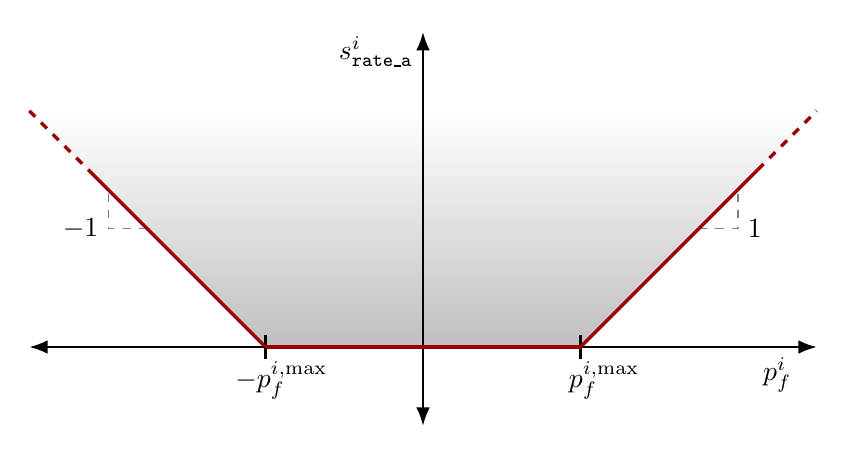
\begin{tikzpicture}[>={Latex},
redline/.style={red!60!black, very thick},
slopeline/.style={gray, dashed},
]

% axes
\draw[thick,<->] (-5,0) -- (5,0) node[below,pos=0.95] {$p^i_f$};
\draw[thick,<->] (0,-1) -- (0,4) node[left,pos=0.95] {$s^i_{\code{rate\_a}}$};

%ticks
\draw[thick] (-2,0.15) -- (-2, -0.15) node[below,xshift=0.2cm, yshift=0.1cm] {$-p^{i,\text{max}}_{f}$};
\draw[thick] (2,0.15) --  (2, -0.15) node[below, yshift=0.1cm, xshift=0.3cm] {$p^{i,\text{max}}_{f}$};

% softlim slope
\draw[slopeline] (-3.5,1.5) -| node[left,black] {$-1$} (-4,2);
\draw[slopeline] (3.5,1.5) -| node[right,black] {$1$} (4,2);

\begin{scope}[on background layer, transparency group]
\shade[left color=gray!50, right color=gray!50, bottom color=gray!50, top color=white]  (-5,3) -- (-2,0) -- (2,0) -- (5,3) -- cycle;
\end{scope}

% limit boundary
\draw[redline, dashed]  (-5,3) -- (-4.25,2.25);
\draw[redline]  (-4.25,2.25) --  (-2,0);
\draw[redline] (-2,0) -- (2,0);
\draw[redline] (2,0) -- (4.25, 2.25);
\draw[redline, dashed] (4.25, 2.25) -- (5,3);


\end{tikzpicture}

\end{document}